%!TEX root = mainfile.tex
%Use Passive tense.
\section{Parameter Values} % (fold)
\label{sec:parameter_values}
	There are also a number of parameters in the Schechter function that must be specified. In order to find suitable values to use, data from a number of different sources has been collected covering several studies. All of the studies that have been performed in the past concern galaxies at lower redshifts than were examined. To get an estimate for the value of each of the parameters at higher redshift, the values found were plotted and the fit extrapolated to cover the era necessary. Since some of the fits demonstrate that these parameters are not constant with time, their evolution shall be incorporated into the calculations.

	The values in the Schechter function that have been fitted are $\alpha$, $M^{*}$ and $\phi^{*}$. The data collected for each of these fits is shown in appendix~\ref{app:parameter_fit_data}.

	\subsection{Parameter Evolution} % (fold)
	\label{sub:parameter_evolution}
		The early stages of the models that were used assumed that the parameters of the Schechter function were static with respect to time. This means that, when iterating over the redshift, the only property that changed was the co-moving volume. This is non-physical since it does not allow for changes in the characteristic mass and characteristic luminosity for different conditions in the universe. In order to improve the model, data from a number of previous studies was collected for three values, the characteristic mass, $M^*$, the Schechter normalisation, $\phi^*$ and the faint end slope parameter, $\alpha$.

		\subsubsection{Linear Parameter Evolution with Redshift} % (fold)
		\label{ssub:linear_parameter_evolution_with_redshift}
			In order to provide useful errors on the fits of the parameters, a technique called the pivot fit method is used to decouple the errors on $y$-intercept and gradient. This involves fitting the data after it has been normalised around the mean value. This normalisation simply involves taking the mean $x$- and $y$-value from each data point so that the graph is centred about the origin. This means that the $y$-intercept is fixed to zero and thus the fitting error applies only to the gradient. Subsequent linear fits shall be treated in this manner, so that errors quoted correspond to the gradient. For clarity of presentation, the data shall be plotted in its original form.

			The graph in Figure~\ref{fig:alpha_evolution} shows the data collected, with the corresponding uncertainties, for the linear parameter, $\alpha$. From this data, a linear fit is taken. The relevant evolution, then, is governed by the equation $\alpha = -0.015z - 1.664$.
			\begin{figure}[!htbp]
				\begin{minipage}[c]{0.5\linewidth}
					\centering
						\begingroup\endlinechar=-1
							\resizebox{\textwidth}{!}{%
								% GNUPLOT: LaTeX picture with Postscript
\begingroup
  \makeatletter
  \providecommand\color[2][]{%
    \GenericError{(gnuplot) \space\space\space\@spaces}{%
      Package color not loaded in conjunction with
      terminal option `colourtext'%
    }{See the gnuplot documentation for explanation.%
    }{Either use 'blacktext' in gnuplot or load the package
      color.sty in LaTeX.}%
    \renewcommand\color[2][]{}%
  }%
  \providecommand\includegraphics[2][]{%
    \GenericError{(gnuplot) \space\space\space\@spaces}{%
      Package graphicx or graphics not loaded%
    }{See the gnuplot documentation for explanation.%
    }{The gnuplot epslatex terminal needs graphicx.sty or graphics.sty.}%
    \renewcommand\includegraphics[2][]{}%
  }%
  \providecommand\rotatebox[2]{#2}%
  \@ifundefined{ifGPcolor}{%
    \newif\ifGPcolor
    \GPcolortrue
  }{}%
  \@ifundefined{ifGPblacktext}{%
    \newif\ifGPblacktext
    \GPblacktexttrue
  }{}%
  % define a \g@addto@macro without @ in the name:
  \let\gplgaddtomacro\g@addto@macro
  % define empty templates for all commands taking text:
  \gdef\gplbacktext{}%
  \gdef\gplfronttext{}%
  \makeatother
  \ifGPblacktext
    % no textcolor at all
    \def\colorrgb#1{}%
    \def\colorgray#1{}%
  \else
    % gray or color?
    \ifGPcolor
      \def\colorrgb#1{\color[rgb]{#1}}%
      \def\colorgray#1{\color[gray]{#1}}%
      \expandafter\def\csname LTw\endcsname{\color{white}}%
      \expandafter\def\csname LTb\endcsname{\color{black}}%
      \expandafter\def\csname LTa\endcsname{\color{black}}%
      \expandafter\def\csname LT0\endcsname{\color[rgb]{1,0,0}}%
      \expandafter\def\csname LT1\endcsname{\color[rgb]{0,1,0}}%
      \expandafter\def\csname LT2\endcsname{\color[rgb]{0,0,1}}%
      \expandafter\def\csname LT3\endcsname{\color[rgb]{1,0,1}}%
      \expandafter\def\csname LT4\endcsname{\color[rgb]{0,1,1}}%
      \expandafter\def\csname LT5\endcsname{\color[rgb]{1,1,0}}%
      \expandafter\def\csname LT6\endcsname{\color[rgb]{0,0,0}}%
      \expandafter\def\csname LT7\endcsname{\color[rgb]{1,0.3,0}}%
      \expandafter\def\csname LT8\endcsname{\color[rgb]{0.5,0.5,0.5}}%
    \else
      % gray
      \def\colorrgb#1{\color{black}}%
      \def\colorgray#1{\color[gray]{#1}}%
      \expandafter\def\csname LTw\endcsname{\color{white}}%
      \expandafter\def\csname LTb\endcsname{\color{black}}%
      \expandafter\def\csname LTa\endcsname{\color{black}}%
      \expandafter\def\csname LT0\endcsname{\color{black}}%
      \expandafter\def\csname LT1\endcsname{\color{black}}%
      \expandafter\def\csname LT2\endcsname{\color{black}}%
      \expandafter\def\csname LT3\endcsname{\color{black}}%
      \expandafter\def\csname LT4\endcsname{\color{black}}%
      \expandafter\def\csname LT5\endcsname{\color{black}}%
      \expandafter\def\csname LT6\endcsname{\color{black}}%
      \expandafter\def\csname LT7\endcsname{\color{black}}%
      \expandafter\def\csname LT8\endcsname{\color{black}}%
    \fi
  \fi
  \setlength{\unitlength}{0.0500bp}%
  \begin{picture}(7200.00,4320.00)%
    \gplgaddtomacro\gplbacktext{%
      \put(747,915){\makebox(0,0)[r]{\strut{}-2.2}}%
      \put(747,1555){\makebox(0,0)[r]{\strut{}-2}}%
      \put(747,2195){\makebox(0,0)[r]{\strut{}-1.8}}%
      \put(747,2835){\makebox(0,0)[r]{\strut{}-1.6}}%
      \put(747,3475){\makebox(0,0)[r]{\strut{}-1.4}}%
      \put(747,4115){\makebox(0,0)[r]{\strut{}-1.2}}%
      \put(849,409){\makebox(0,0){\strut{} 0}}%
      \put(2058,409){\makebox(0,0){\strut{} 2}}%
      \put(3267,409){\makebox(0,0){\strut{} 4}}%
      \put(4475,409){\makebox(0,0){\strut{} 6}}%
      \put(5684,409){\makebox(0,0){\strut{} 8}}%
      \put(6893,409){\makebox(0,0){\strut{} 10}}%
      \csname LTb\endcsname%
      \put(144,2355){\rotatebox{-270}{\makebox(0,0){\strut{}Faint End Slope ($\alpha$)}}}%
      \csname LTb\endcsname%
      \put(3871,130){\makebox(0,0){\strut{}Redshift ($z$)}}%
      \put(3871,4022){\makebox(0,0){\strut{}}}%
    }%
    \gplgaddtomacro\gplfronttext{%
      \csname LTb\endcsname%
      \put(3297,762){\makebox(0,0)[r]{\strut{}$f(x) = -0.015x + -1.664$}}%
    }%
    \gplbacktext
    \put(0,0){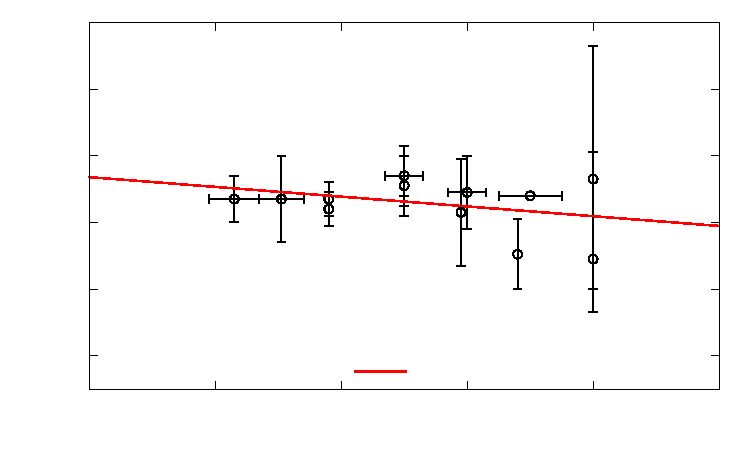
\includegraphics{GRAPH_Parameter_Fit_alpha_linear}}%
    \gplfronttext
  \end{picture}%
\endgroup

							}\endgroup
				\end{minipage}
				\begin{minipage}[c]{0.5\linewidth}
					\centering
						\begingroup\endlinechar=-1
							\resizebox{\textwidth}{!}{%
								% GNUPLOT: LaTeX picture with Postscript
\begingroup
  \makeatletter
  \providecommand\color[2][]{%
    \GenericError{(gnuplot) \space\space\space\@spaces}{%
      Package color not loaded in conjunction with
      terminal option `colourtext'%
    }{See the gnuplot documentation for explanation.%
    }{Either use 'blacktext' in gnuplot or load the package
      color.sty in LaTeX.}%
    \renewcommand\color[2][]{}%
  }%
  \providecommand\includegraphics[2][]{%
    \GenericError{(gnuplot) \space\space\space\@spaces}{%
      Package graphicx or graphics not loaded%
    }{See the gnuplot documentation for explanation.%
    }{The gnuplot epslatex terminal needs graphicx.sty or graphics.sty.}%
    \renewcommand\includegraphics[2][]{}%
  }%
  \providecommand\rotatebox[2]{#2}%
  \@ifundefined{ifGPcolor}{%
    \newif\ifGPcolor
    \GPcolortrue
  }{}%
  \@ifundefined{ifGPblacktext}{%
    \newif\ifGPblacktext
    \GPblacktexttrue
  }{}%
  % define a \g@addto@macro without @ in the name:
  \let\gplgaddtomacro\g@addto@macro
  % define empty templates for all commands taking text:
  \gdef\gplbacktext{}%
  \gdef\gplfronttext{}%
  \makeatother
  \ifGPblacktext
    % no textcolor at all
    \def\colorrgb#1{}%
    \def\colorgray#1{}%
  \else
    % gray or color?
    \ifGPcolor
      \def\colorrgb#1{\color[rgb]{#1}}%
      \def\colorgray#1{\color[gray]{#1}}%
      \expandafter\def\csname LTw\endcsname{\color{white}}%
      \expandafter\def\csname LTb\endcsname{\color{black}}%
      \expandafter\def\csname LTa\endcsname{\color{black}}%
      \expandafter\def\csname LT0\endcsname{\color[rgb]{1,0,0}}%
      \expandafter\def\csname LT1\endcsname{\color[rgb]{0,1,0}}%
      \expandafter\def\csname LT2\endcsname{\color[rgb]{0,0,1}}%
      \expandafter\def\csname LT3\endcsname{\color[rgb]{1,0,1}}%
      \expandafter\def\csname LT4\endcsname{\color[rgb]{0,1,1}}%
      \expandafter\def\csname LT5\endcsname{\color[rgb]{1,1,0}}%
      \expandafter\def\csname LT6\endcsname{\color[rgb]{0,0,0}}%
      \expandafter\def\csname LT7\endcsname{\color[rgb]{1,0.3,0}}%
      \expandafter\def\csname LT8\endcsname{\color[rgb]{0.5,0.5,0.5}}%
    \else
      % gray
      \def\colorrgb#1{\color{black}}%
      \def\colorgray#1{\color[gray]{#1}}%
      \expandafter\def\csname LTw\endcsname{\color{white}}%
      \expandafter\def\csname LTb\endcsname{\color{black}}%
      \expandafter\def\csname LTa\endcsname{\color{black}}%
      \expandafter\def\csname LT0\endcsname{\color{black}}%
      \expandafter\def\csname LT1\endcsname{\color{black}}%
      \expandafter\def\csname LT2\endcsname{\color{black}}%
      \expandafter\def\csname LT3\endcsname{\color{black}}%
      \expandafter\def\csname LT4\endcsname{\color{black}}%
      \expandafter\def\csname LT5\endcsname{\color{black}}%
      \expandafter\def\csname LT6\endcsname{\color{black}}%
      \expandafter\def\csname LT7\endcsname{\color{black}}%
      \expandafter\def\csname LT8\endcsname{\color{black}}%
    \fi
  \fi
  \setlength{\unitlength}{0.0500bp}%
  \begin{picture}(7200.00,4320.00)%
    \gplgaddtomacro\gplbacktext{%
      \put(849,595){\makebox(0,0)[r]{\strut{}-2.1}}%
      \put(849,947){\makebox(0,0)[r]{\strut{}-2.05}}%
      \put(849,1299){\makebox(0,0)[r]{\strut{}-2}}%
      \put(849,1651){\makebox(0,0)[r]{\strut{}-1.95}}%
      \put(849,2003){\makebox(0,0)[r]{\strut{}-1.9}}%
      \put(849,2355){\makebox(0,0)[r]{\strut{}-1.85}}%
      \put(849,2707){\makebox(0,0)[r]{\strut{}-1.8}}%
      \put(849,3059){\makebox(0,0)[r]{\strut{}-1.75}}%
      \put(849,3411){\makebox(0,0)[r]{\strut{}-1.7}}%
      \put(849,3763){\makebox(0,0)[r]{\strut{}-1.65}}%
      \put(849,4115){\makebox(0,0)[r]{\strut{}-1.6}}%
      \put(951,409){\makebox(0,0){\strut{} 0}}%
      \put(1611,409){\makebox(0,0){\strut{} 2}}%
      \put(2271,409){\makebox(0,0){\strut{} 4}}%
      \put(2932,409){\makebox(0,0){\strut{} 6}}%
      \put(3592,409){\makebox(0,0){\strut{} 8}}%
      \put(4252,409){\makebox(0,0){\strut{} 10}}%
      \put(4912,409){\makebox(0,0){\strut{} 12}}%
      \put(5573,409){\makebox(0,0){\strut{} 14}}%
      \put(6233,409){\makebox(0,0){\strut{} 16}}%
      \put(6893,409){\makebox(0,0){\strut{} 18}}%
      \csname LTb\endcsname%
      \put(144,2355){\rotatebox{-270}{\makebox(0,0){\strut{}Faint End Slope ($\alpha$)}}}%
      \csname LTb\endcsname%
      \put(3922,130){\makebox(0,0){\strut{}Redshift ($z$)}}%
      \put(3922,4022){\makebox(0,0){\strut{}}}%
    }%
    \gplgaddtomacro\gplfronttext{%
      \csname LTb\endcsname%
      \put(2906,1206){\makebox(0,0)[r]{\strut{}Predicated Value of $\alpha$}}%
      \csname LTb\endcsname%
      \put(2906,1020){\makebox(0,0)[r]{\strut{}Upper Limit}}%
      \csname LTb\endcsname%
      \put(2906,834){\makebox(0,0)[r]{\strut{}Lower Limit}}%
    }%
    \gplbacktext
    \put(0,0){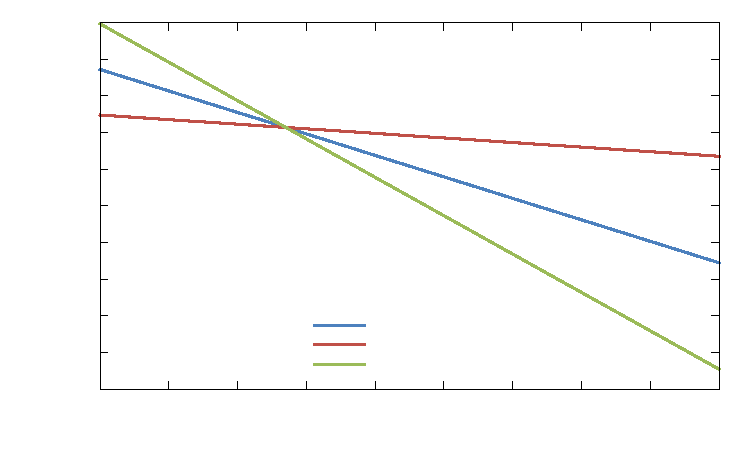
\includegraphics{GRAPH_Parameter_Fit_alpha_bounds}}%
    \gplfronttext
  \end{picture}%
\endgroup

							}\endgroup
				\end{minipage}
				\caption{The evolution of $\alpha$ as a function of redshift according to past observational studies, left. Using the upper and lower limits of the parameter fit, the bounds of the value of $\alpha$ are plotted, right.\label{fig:alpha_evolution}}
			\end{figure}

			Figure~\ref{fig:phi_evolution} shows the data for the evolution of the normalisation parameter $\phi^{*}$. This value is known to be never less than zero. For this reason, coupled with an attempt to reduce the errors as far as possible, an exponential decrease with redshift was chosen. Although the errors for this fit are large, because of the errors on the data points, the region of concern, high redshift greater than 6, this evolution can be approximated to zero. In other words, during the times that is being considered, it can be approximated that there was no change in the value of the normalisation parameter, $\phi^*$.
			% \begin{figure}[!htbp]
			% 	\centering
			% 		\begingroup\endlinechar=-1
			% 			\resizebox{0.6\textwidth}{!}{%
			% 				% GNUPLOT: LaTeX picture with Postscript
\begingroup
  \makeatletter
  \providecommand\color[2][]{%
    \GenericError{(gnuplot) \space\space\space\@spaces}{%
      Package color not loaded in conjunction with
      terminal option `colourtext'%
    }{See the gnuplot documentation for explanation.%
    }{Either use 'blacktext' in gnuplot or load the package
      color.sty in LaTeX.}%
    \renewcommand\color[2][]{}%
  }%
  \providecommand\includegraphics[2][]{%
    \GenericError{(gnuplot) \space\space\space\@spaces}{%
      Package graphicx or graphics not loaded%
    }{See the gnuplot documentation for explanation.%
    }{The gnuplot epslatex terminal needs graphicx.sty or graphics.sty.}%
    \renewcommand\includegraphics[2][]{}%
  }%
  \providecommand\rotatebox[2]{#2}%
  \@ifundefined{ifGPcolor}{%
    \newif\ifGPcolor
    \GPcolortrue
  }{}%
  \@ifundefined{ifGPblacktext}{%
    \newif\ifGPblacktext
    \GPblacktexttrue
  }{}%
  % define a \g@addto@macro without @ in the name:
  \let\gplgaddtomacro\g@addto@macro
  % define empty templates for all commands taking text:
  \gdef\gplbacktext{}%
  \gdef\gplfronttext{}%
  \makeatother
  \ifGPblacktext
    % no textcolor at all
    \def\colorrgb#1{}%
    \def\colorgray#1{}%
  \else
    % gray or color?
    \ifGPcolor
      \def\colorrgb#1{\color[rgb]{#1}}%
      \def\colorgray#1{\color[gray]{#1}}%
      \expandafter\def\csname LTw\endcsname{\color{white}}%
      \expandafter\def\csname LTb\endcsname{\color{black}}%
      \expandafter\def\csname LTa\endcsname{\color{black}}%
      \expandafter\def\csname LT0\endcsname{\color[rgb]{1,0,0}}%
      \expandafter\def\csname LT1\endcsname{\color[rgb]{0,1,0}}%
      \expandafter\def\csname LT2\endcsname{\color[rgb]{0,0,1}}%
      \expandafter\def\csname LT3\endcsname{\color[rgb]{1,0,1}}%
      \expandafter\def\csname LT4\endcsname{\color[rgb]{0,1,1}}%
      \expandafter\def\csname LT5\endcsname{\color[rgb]{1,1,0}}%
      \expandafter\def\csname LT6\endcsname{\color[rgb]{0,0,0}}%
      \expandafter\def\csname LT7\endcsname{\color[rgb]{1,0.3,0}}%
      \expandafter\def\csname LT8\endcsname{\color[rgb]{0.5,0.5,0.5}}%
    \else
      % gray
      \def\colorrgb#1{\color{black}}%
      \def\colorgray#1{\color[gray]{#1}}%
      \expandafter\def\csname LTw\endcsname{\color{white}}%
      \expandafter\def\csname LTb\endcsname{\color{black}}%
      \expandafter\def\csname LTa\endcsname{\color{black}}%
      \expandafter\def\csname LT0\endcsname{\color{black}}%
      \expandafter\def\csname LT1\endcsname{\color{black}}%
      \expandafter\def\csname LT2\endcsname{\color{black}}%
      \expandafter\def\csname LT3\endcsname{\color{black}}%
      \expandafter\def\csname LT4\endcsname{\color{black}}%
      \expandafter\def\csname LT5\endcsname{\color{black}}%
      \expandafter\def\csname LT6\endcsname{\color{black}}%
      \expandafter\def\csname LT7\endcsname{\color{black}}%
      \expandafter\def\csname LT8\endcsname{\color{black}}%
    \fi
  \fi
  \setlength{\unitlength}{0.0500bp}%
  \begin{picture}(7200.00,4320.00)%
    \gplgaddtomacro\gplbacktext{%
      \put(1053,595){\makebox(0,0)[r]{\strut{} 0}}%
      \put(1053,947){\makebox(0,0)[r]{\strut{} 0.0005}}%
      \put(1053,1299){\makebox(0,0)[r]{\strut{} 0.001}}%
      \put(1053,1651){\makebox(0,0)[r]{\strut{} 0.0015}}%
      \put(1053,2003){\makebox(0,0)[r]{\strut{} 0.002}}%
      \put(1053,2355){\makebox(0,0)[r]{\strut{} 0.0025}}%
      \put(1053,2707){\makebox(0,0)[r]{\strut{} 0.003}}%
      \put(1053,3059){\makebox(0,0)[r]{\strut{} 0.0035}}%
      \put(1053,3411){\makebox(0,0)[r]{\strut{} 0.004}}%
      \put(1053,3763){\makebox(0,0)[r]{\strut{} 0.0045}}%
      \put(1053,4115){\makebox(0,0)[r]{\strut{} 0.005}}%
      \put(1155,409){\makebox(0,0){\strut{} 0}}%
      \put(2303,409){\makebox(0,0){\strut{} 2}}%
      \put(3450,409){\makebox(0,0){\strut{} 4}}%
      \put(4598,409){\makebox(0,0){\strut{} 6}}%
      \put(5745,409){\makebox(0,0){\strut{} 8}}%
      \put(6893,409){\makebox(0,0){\strut{} 10}}%
      \csname LTb\endcsname%
      \put(144,2355){\rotatebox{-270}{\makebox(0,0){\strut{}Normalisation ($\phi^{*}$)}}}%
      \csname LTb\endcsname%
      \put(4024,130){\makebox(0,0){\strut{}Redshift ($z$)}}%
      \put(4024,4022){\makebox(0,0){\strut{}}}%
    }%
    \gplgaddtomacro\gplfronttext{%
      \csname LTb\endcsname%
      \put(6105,3948){\makebox(0,0)[r]{\strut{}$f(x) = 0.052e^{-1.487x} + 0.001$}}%
    }%
    \gplbacktext
    \put(0,0){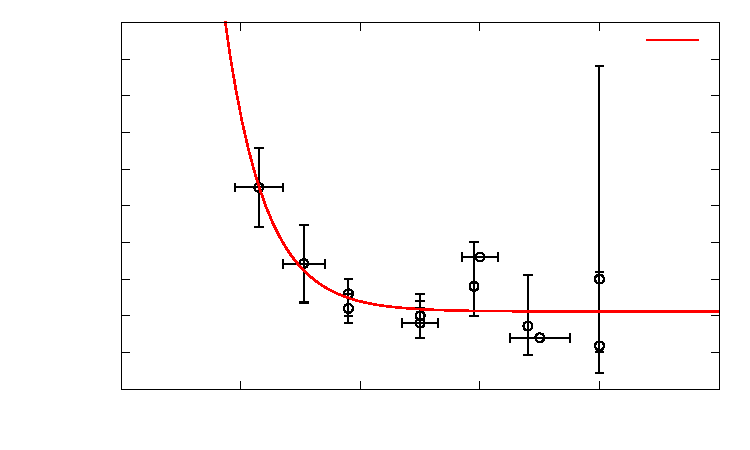
\includegraphics{GRAPH_Parameter_Fit_phi-star_exponential}}%
    \gplfronttext
  \end{picture}%
\endgroup

			% 			}\endgroup
			% 	\caption{The evolution of $\phi^{*}$ as a function of redshift according to past observational studies.\label{fig:phi_evolution}}
			% \end{figure}
			\begin{figure}[!htbp]
				\begin{minipage}[c]{0.5\linewidth}
					\centering
						\begingroup\endlinechar=-1
							\resizebox{\textwidth}{!}{%
								% GNUPLOT: LaTeX picture with Postscript
\begingroup
  \makeatletter
  \providecommand\color[2][]{%
    \GenericError{(gnuplot) \space\space\space\@spaces}{%
      Package color not loaded in conjunction with
      terminal option `colourtext'%
    }{See the gnuplot documentation for explanation.%
    }{Either use 'blacktext' in gnuplot or load the package
      color.sty in LaTeX.}%
    \renewcommand\color[2][]{}%
  }%
  \providecommand\includegraphics[2][]{%
    \GenericError{(gnuplot) \space\space\space\@spaces}{%
      Package graphicx or graphics not loaded%
    }{See the gnuplot documentation for explanation.%
    }{The gnuplot epslatex terminal needs graphicx.sty or graphics.sty.}%
    \renewcommand\includegraphics[2][]{}%
  }%
  \providecommand\rotatebox[2]{#2}%
  \@ifundefined{ifGPcolor}{%
    \newif\ifGPcolor
    \GPcolortrue
  }{}%
  \@ifundefined{ifGPblacktext}{%
    \newif\ifGPblacktext
    \GPblacktexttrue
  }{}%
  % define a \g@addto@macro without @ in the name:
  \let\gplgaddtomacro\g@addto@macro
  % define empty templates for all commands taking text:
  \gdef\gplbacktext{}%
  \gdef\gplfronttext{}%
  \makeatother
  \ifGPblacktext
    % no textcolor at all
    \def\colorrgb#1{}%
    \def\colorgray#1{}%
  \else
    % gray or color?
    \ifGPcolor
      \def\colorrgb#1{\color[rgb]{#1}}%
      \def\colorgray#1{\color[gray]{#1}}%
      \expandafter\def\csname LTw\endcsname{\color{white}}%
      \expandafter\def\csname LTb\endcsname{\color{black}}%
      \expandafter\def\csname LTa\endcsname{\color{black}}%
      \expandafter\def\csname LT0\endcsname{\color[rgb]{1,0,0}}%
      \expandafter\def\csname LT1\endcsname{\color[rgb]{0,1,0}}%
      \expandafter\def\csname LT2\endcsname{\color[rgb]{0,0,1}}%
      \expandafter\def\csname LT3\endcsname{\color[rgb]{1,0,1}}%
      \expandafter\def\csname LT4\endcsname{\color[rgb]{0,1,1}}%
      \expandafter\def\csname LT5\endcsname{\color[rgb]{1,1,0}}%
      \expandafter\def\csname LT6\endcsname{\color[rgb]{0,0,0}}%
      \expandafter\def\csname LT7\endcsname{\color[rgb]{1,0.3,0}}%
      \expandafter\def\csname LT8\endcsname{\color[rgb]{0.5,0.5,0.5}}%
    \else
      % gray
      \def\colorrgb#1{\color{black}}%
      \def\colorgray#1{\color[gray]{#1}}%
      \expandafter\def\csname LTw\endcsname{\color{white}}%
      \expandafter\def\csname LTb\endcsname{\color{black}}%
      \expandafter\def\csname LTa\endcsname{\color{black}}%
      \expandafter\def\csname LT0\endcsname{\color{black}}%
      \expandafter\def\csname LT1\endcsname{\color{black}}%
      \expandafter\def\csname LT2\endcsname{\color{black}}%
      \expandafter\def\csname LT3\endcsname{\color{black}}%
      \expandafter\def\csname LT4\endcsname{\color{black}}%
      \expandafter\def\csname LT5\endcsname{\color{black}}%
      \expandafter\def\csname LT6\endcsname{\color{black}}%
      \expandafter\def\csname LT7\endcsname{\color{black}}%
      \expandafter\def\csname LT8\endcsname{\color{black}}%
    \fi
  \fi
  \setlength{\unitlength}{0.0500bp}%
  \begin{picture}(7200.00,4320.00)%
    \gplgaddtomacro\gplbacktext{%
      \put(1053,595){\makebox(0,0)[r]{\strut{} 0}}%
      \put(1053,947){\makebox(0,0)[r]{\strut{} 0.0005}}%
      \put(1053,1299){\makebox(0,0)[r]{\strut{} 0.001}}%
      \put(1053,1651){\makebox(0,0)[r]{\strut{} 0.0015}}%
      \put(1053,2003){\makebox(0,0)[r]{\strut{} 0.002}}%
      \put(1053,2355){\makebox(0,0)[r]{\strut{} 0.0025}}%
      \put(1053,2707){\makebox(0,0)[r]{\strut{} 0.003}}%
      \put(1053,3059){\makebox(0,0)[r]{\strut{} 0.0035}}%
      \put(1053,3411){\makebox(0,0)[r]{\strut{} 0.004}}%
      \put(1053,3763){\makebox(0,0)[r]{\strut{} 0.0045}}%
      \put(1053,4115){\makebox(0,0)[r]{\strut{} 0.005}}%
      \put(1155,409){\makebox(0,0){\strut{} 0}}%
      \put(2303,409){\makebox(0,0){\strut{} 2}}%
      \put(3450,409){\makebox(0,0){\strut{} 4}}%
      \put(4598,409){\makebox(0,0){\strut{} 6}}%
      \put(5745,409){\makebox(0,0){\strut{} 8}}%
      \put(6893,409){\makebox(0,0){\strut{} 10}}%
      \csname LTb\endcsname%
      \put(144,2355){\rotatebox{-270}{\makebox(0,0){\strut{}Normalisation ($\phi^{*}$)}}}%
      \csname LTb\endcsname%
      \put(4024,130){\makebox(0,0){\strut{}Redshift ($z$)}}%
      \put(4024,4022){\makebox(0,0){\strut{}}}%
    }%
    \gplgaddtomacro\gplfronttext{%
      \csname LTb\endcsname%
      \put(6105,3948){\makebox(0,0)[r]{\strut{}$f(x) = 0.052e^{-1.487x} + 0.001$}}%
    }%
    \gplbacktext
    \put(0,0){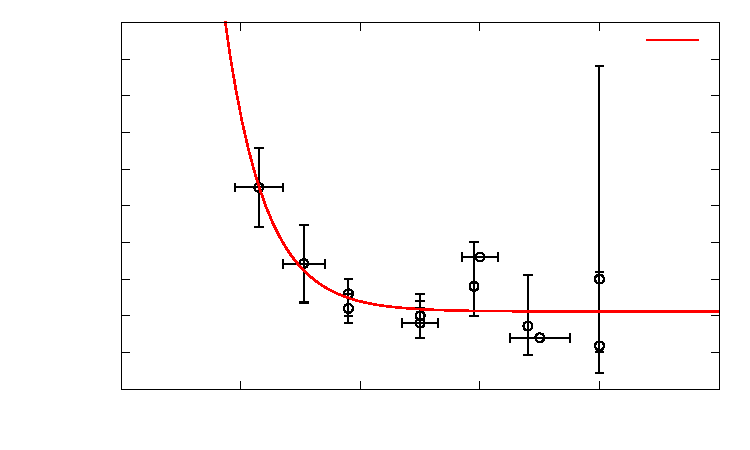
\includegraphics{GRAPH_Parameter_Fit_phi-star_exponential}}%
    \gplfronttext
  \end{picture}%
\endgroup

							}\endgroup
				\end{minipage}
				\begin{minipage}[c]{0.5\linewidth}
					\centering
						\begingroup\endlinechar=-1
							\resizebox{\textwidth}{!}{%
								% GNUPLOT: LaTeX picture with Postscript
\begingroup
  \makeatletter
  \providecommand\color[2][]{%
    \GenericError{(gnuplot) \space\space\space\@spaces}{%
      Package color not loaded in conjunction with
      terminal option `colourtext'%
    }{See the gnuplot documentation for explanation.%
    }{Either use 'blacktext' in gnuplot or load the package
      color.sty in LaTeX.}%
    \renewcommand\color[2][]{}%
  }%
  \providecommand\includegraphics[2][]{%
    \GenericError{(gnuplot) \space\space\space\@spaces}{%
      Package graphicx or graphics not loaded%
    }{See the gnuplot documentation for explanation.%
    }{The gnuplot epslatex terminal needs graphicx.sty or graphics.sty.}%
    \renewcommand\includegraphics[2][]{}%
  }%
  \providecommand\rotatebox[2]{#2}%
  \@ifundefined{ifGPcolor}{%
    \newif\ifGPcolor
    \GPcolortrue
  }{}%
  \@ifundefined{ifGPblacktext}{%
    \newif\ifGPblacktext
    \GPblacktexttrue
  }{}%
  % define a \g@addto@macro without @ in the name:
  \let\gplgaddtomacro\g@addto@macro
  % define empty templates for all commands taking text:
  \gdef\gplbacktext{}%
  \gdef\gplfronttext{}%
  \makeatother
  \ifGPblacktext
    % no textcolor at all
    \def\colorrgb#1{}%
    \def\colorgray#1{}%
  \else
    % gray or color?
    \ifGPcolor
      \def\colorrgb#1{\color[rgb]{#1}}%
      \def\colorgray#1{\color[gray]{#1}}%
      \expandafter\def\csname LTw\endcsname{\color{white}}%
      \expandafter\def\csname LTb\endcsname{\color{black}}%
      \expandafter\def\csname LTa\endcsname{\color{black}}%
      \expandafter\def\csname LT0\endcsname{\color[rgb]{1,0,0}}%
      \expandafter\def\csname LT1\endcsname{\color[rgb]{0,1,0}}%
      \expandafter\def\csname LT2\endcsname{\color[rgb]{0,0,1}}%
      \expandafter\def\csname LT3\endcsname{\color[rgb]{1,0,1}}%
      \expandafter\def\csname LT4\endcsname{\color[rgb]{0,1,1}}%
      \expandafter\def\csname LT5\endcsname{\color[rgb]{1,1,0}}%
      \expandafter\def\csname LT6\endcsname{\color[rgb]{0,0,0}}%
      \expandafter\def\csname LT7\endcsname{\color[rgb]{1,0.3,0}}%
      \expandafter\def\csname LT8\endcsname{\color[rgb]{0.5,0.5,0.5}}%
    \else
      % gray
      \def\colorrgb#1{\color{black}}%
      \def\colorgray#1{\color[gray]{#1}}%
      \expandafter\def\csname LTw\endcsname{\color{white}}%
      \expandafter\def\csname LTb\endcsname{\color{black}}%
      \expandafter\def\csname LTa\endcsname{\color{black}}%
      \expandafter\def\csname LT0\endcsname{\color{black}}%
      \expandafter\def\csname LT1\endcsname{\color{black}}%
      \expandafter\def\csname LT2\endcsname{\color{black}}%
      \expandafter\def\csname LT3\endcsname{\color{black}}%
      \expandafter\def\csname LT4\endcsname{\color{black}}%
      \expandafter\def\csname LT5\endcsname{\color{black}}%
      \expandafter\def\csname LT6\endcsname{\color{black}}%
      \expandafter\def\csname LT7\endcsname{\color{black}}%
      \expandafter\def\csname LT8\endcsname{\color{black}}%
    \fi
  \fi
  \setlength{\unitlength}{0.0500bp}%
  \begin{picture}(7200.00,4320.00)%
    \gplgaddtomacro\gplbacktext{%
      \put(849,595){\makebox(0,0)[r]{\strut{}-0.05}}%
      \put(849,1299){\makebox(0,0)[r]{\strut{} 0}}%
      \put(849,2003){\makebox(0,0)[r]{\strut{} 0.05}}%
      \put(849,2707){\makebox(0,0)[r]{\strut{} 0.1}}%
      \put(849,3411){\makebox(0,0)[r]{\strut{} 0.15}}%
      \put(849,4115){\makebox(0,0)[r]{\strut{} 0.2}}%
      \put(951,409){\makebox(0,0){\strut{} 0}}%
      \put(1611,409){\makebox(0,0){\strut{} 2}}%
      \put(2271,409){\makebox(0,0){\strut{} 4}}%
      \put(2932,409){\makebox(0,0){\strut{} 6}}%
      \put(3592,409){\makebox(0,0){\strut{} 8}}%
      \put(4252,409){\makebox(0,0){\strut{} 10}}%
      \put(4912,409){\makebox(0,0){\strut{} 12}}%
      \put(5573,409){\makebox(0,0){\strut{} 14}}%
      \put(6233,409){\makebox(0,0){\strut{} 16}}%
      \put(6893,409){\makebox(0,0){\strut{} 18}}%
      \csname LTb\endcsname%
      \put(144,2355){\rotatebox{-270}{\makebox(0,0){\strut{}Normalisation ($\phi^*$)}}}%
      \csname LTb\endcsname%
      \put(3922,130){\makebox(0,0){\strut{}Redshift ($z$)}}%
      \put(3922,4022){\makebox(0,0){\strut{}}}%
    }%
    \gplgaddtomacro\gplfronttext{%
      \csname LTb\endcsname%
      \put(5877,3740){\makebox(0,0)[r]{\strut{}Predicated Value of $\phi^*$}}%
      \csname LTb\endcsname%
      \put(5877,3554){\makebox(0,0)[r]{\strut{}Upper Limit}}%
      \csname LTb\endcsname%
      \put(5877,3368){\makebox(0,0)[r]{\strut{}Lower Limit}}%
    }%
    \gplbacktext
    \put(0,0){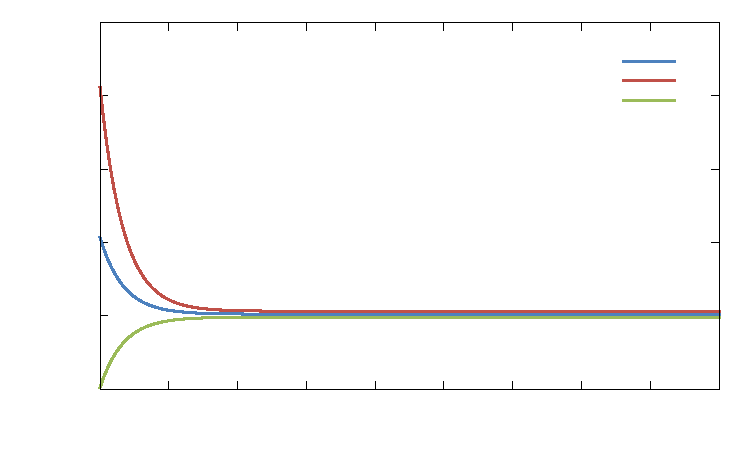
\includegraphics{GRAPH_Parameter_Fit_phi-star_bounds}}%
    \gplfronttext
  \end{picture}%
\endgroup

							}\endgroup
				\end{minipage}
				\caption{The evolution of $\phi^{*}$ as a function of redshift according to past observational studies. Using the upper and lower limits of the parameter fit, the bounds of the value of $\phi^*$ are plotted, right.\label{fig:phi_evolution}}
			\end{figure}

			The final parameter is the characteristic magnitude, $M^*$. It was determined that a linear fit was best again and so the pivot method was used to reduce the error. The final equation used was $M^* = 0.221z - 21.642$, shown in Figure~\ref{fig:m-star_evolution}.
			% \begin{figure}[!htbp]
			% 	\centering
			% 		\begingroup\endlinechar=-1
			% 			\resizebox{0.6\textwidth}{!}{%
			% 				% GNUPLOT: LaTeX picture with Postscript
\begingroup
  \makeatletter
  \providecommand\color[2][]{%
    \GenericError{(gnuplot) \space\space\space\@spaces}{%
      Package color not loaded in conjunction with
      terminal option `colourtext'%
    }{See the gnuplot documentation for explanation.%
    }{Either use 'blacktext' in gnuplot or load the package
      color.sty in LaTeX.}%
    \renewcommand\color[2][]{}%
  }%
  \providecommand\includegraphics[2][]{%
    \GenericError{(gnuplot) \space\space\space\@spaces}{%
      Package graphicx or graphics not loaded%
    }{See the gnuplot documentation for explanation.%
    }{The gnuplot epslatex terminal needs graphicx.sty or graphics.sty.}%
    \renewcommand\includegraphics[2][]{}%
  }%
  \providecommand\rotatebox[2]{#2}%
  \@ifundefined{ifGPcolor}{%
    \newif\ifGPcolor
    \GPcolortrue
  }{}%
  \@ifundefined{ifGPblacktext}{%
    \newif\ifGPblacktext
    \GPblacktexttrue
  }{}%
  % define a \g@addto@macro without @ in the name:
  \let\gplgaddtomacro\g@addto@macro
  % define empty templates for all commands taking text:
  \gdef\gplbacktext{}%
  \gdef\gplfronttext{}%
  \makeatother
  \ifGPblacktext
    % no textcolor at all
    \def\colorrgb#1{}%
    \def\colorgray#1{}%
  \else
    % gray or color?
    \ifGPcolor
      \def\colorrgb#1{\color[rgb]{#1}}%
      \def\colorgray#1{\color[gray]{#1}}%
      \expandafter\def\csname LTw\endcsname{\color{white}}%
      \expandafter\def\csname LTb\endcsname{\color{black}}%
      \expandafter\def\csname LTa\endcsname{\color{black}}%
      \expandafter\def\csname LT0\endcsname{\color[rgb]{1,0,0}}%
      \expandafter\def\csname LT1\endcsname{\color[rgb]{0,1,0}}%
      \expandafter\def\csname LT2\endcsname{\color[rgb]{0,0,1}}%
      \expandafter\def\csname LT3\endcsname{\color[rgb]{1,0,1}}%
      \expandafter\def\csname LT4\endcsname{\color[rgb]{0,1,1}}%
      \expandafter\def\csname LT5\endcsname{\color[rgb]{1,1,0}}%
      \expandafter\def\csname LT6\endcsname{\color[rgb]{0,0,0}}%
      \expandafter\def\csname LT7\endcsname{\color[rgb]{1,0.3,0}}%
      \expandafter\def\csname LT8\endcsname{\color[rgb]{0.5,0.5,0.5}}%
    \else
      % gray
      \def\colorrgb#1{\color{black}}%
      \def\colorgray#1{\color[gray]{#1}}%
      \expandafter\def\csname LTw\endcsname{\color{white}}%
      \expandafter\def\csname LTb\endcsname{\color{black}}%
      \expandafter\def\csname LTa\endcsname{\color{black}}%
      \expandafter\def\csname LT0\endcsname{\color{black}}%
      \expandafter\def\csname LT1\endcsname{\color{black}}%
      \expandafter\def\csname LT2\endcsname{\color{black}}%
      \expandafter\def\csname LT3\endcsname{\color{black}}%
      \expandafter\def\csname LT4\endcsname{\color{black}}%
      \expandafter\def\csname LT5\endcsname{\color{black}}%
      \expandafter\def\csname LT6\endcsname{\color{black}}%
      \expandafter\def\csname LT7\endcsname{\color{black}}%
      \expandafter\def\csname LT8\endcsname{\color{black}}%
    \fi
  \fi
  \setlength{\unitlength}{0.0500bp}%
  \begin{picture}(7200.00,4320.00)%
    \gplgaddtomacro\gplbacktext{%
      \put(849,595){\makebox(0,0)[r]{\strut{}-22}}%
      \put(849,1098){\makebox(0,0)[r]{\strut{}-21.5}}%
      \put(849,1601){\makebox(0,0)[r]{\strut{}-21}}%
      \put(849,2104){\makebox(0,0)[r]{\strut{}-20.5}}%
      \put(849,2606){\makebox(0,0)[r]{\strut{}-20}}%
      \put(849,3109){\makebox(0,0)[r]{\strut{}-19.5}}%
      \put(849,3612){\makebox(0,0)[r]{\strut{}-19}}%
      \put(849,4115){\makebox(0,0)[r]{\strut{}-18.5}}%
      \put(951,409){\makebox(0,0){\strut{} 0}}%
      \put(2139,409){\makebox(0,0){\strut{} 2}}%
      \put(3328,409){\makebox(0,0){\strut{} 4}}%
      \put(4516,409){\makebox(0,0){\strut{} 6}}%
      \put(5705,409){\makebox(0,0){\strut{} 8}}%
      \put(6893,409){\makebox(0,0){\strut{} 10}}%
      \csname LTb\endcsname%
      \put(144,2355){\rotatebox{-270}{\makebox(0,0){\strut{}Characteristic Magnitude ($M^*$)}}}%
      \csname LTb\endcsname%
      \put(3922,130){\makebox(0,0){\strut{}Redshift ($z$)}}%
      \put(3922,4022){\makebox(0,0){\strut{}}}%
    }%
    \gplgaddtomacro\gplfronttext{%
      \csname LTb\endcsname%
      \put(3399,3948){\makebox(0,0)[r]{\strut{}$f(x) = 0.221x + -21.642$}}%
    }%
    \gplbacktext
    \put(0,0){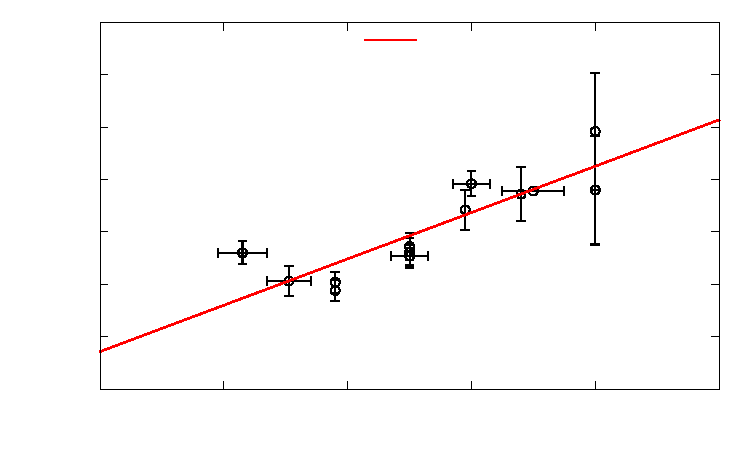
\includegraphics{GRAPH_Parameter_Fit_m-star_linear}}%
    \gplfronttext
  \end{picture}%
\endgroup

			% 			}\endgroup
			% 	\caption{The evolution of $M^{*}$ as a function of redshift according to past observational studies.\label{fig:m-star_evolution}}
			% \end{figure}
			\begin{figure}[!htbp]
				\begin{minipage}[c]{0.5\linewidth}
					\centering
						\begingroup\endlinechar=-1
							\resizebox{\textwidth}{!}{%
								% GNUPLOT: LaTeX picture with Postscript
\begingroup
  \makeatletter
  \providecommand\color[2][]{%
    \GenericError{(gnuplot) \space\space\space\@spaces}{%
      Package color not loaded in conjunction with
      terminal option `colourtext'%
    }{See the gnuplot documentation for explanation.%
    }{Either use 'blacktext' in gnuplot or load the package
      color.sty in LaTeX.}%
    \renewcommand\color[2][]{}%
  }%
  \providecommand\includegraphics[2][]{%
    \GenericError{(gnuplot) \space\space\space\@spaces}{%
      Package graphicx or graphics not loaded%
    }{See the gnuplot documentation for explanation.%
    }{The gnuplot epslatex terminal needs graphicx.sty or graphics.sty.}%
    \renewcommand\includegraphics[2][]{}%
  }%
  \providecommand\rotatebox[2]{#2}%
  \@ifundefined{ifGPcolor}{%
    \newif\ifGPcolor
    \GPcolortrue
  }{}%
  \@ifundefined{ifGPblacktext}{%
    \newif\ifGPblacktext
    \GPblacktexttrue
  }{}%
  % define a \g@addto@macro without @ in the name:
  \let\gplgaddtomacro\g@addto@macro
  % define empty templates for all commands taking text:
  \gdef\gplbacktext{}%
  \gdef\gplfronttext{}%
  \makeatother
  \ifGPblacktext
    % no textcolor at all
    \def\colorrgb#1{}%
    \def\colorgray#1{}%
  \else
    % gray or color?
    \ifGPcolor
      \def\colorrgb#1{\color[rgb]{#1}}%
      \def\colorgray#1{\color[gray]{#1}}%
      \expandafter\def\csname LTw\endcsname{\color{white}}%
      \expandafter\def\csname LTb\endcsname{\color{black}}%
      \expandafter\def\csname LTa\endcsname{\color{black}}%
      \expandafter\def\csname LT0\endcsname{\color[rgb]{1,0,0}}%
      \expandafter\def\csname LT1\endcsname{\color[rgb]{0,1,0}}%
      \expandafter\def\csname LT2\endcsname{\color[rgb]{0,0,1}}%
      \expandafter\def\csname LT3\endcsname{\color[rgb]{1,0,1}}%
      \expandafter\def\csname LT4\endcsname{\color[rgb]{0,1,1}}%
      \expandafter\def\csname LT5\endcsname{\color[rgb]{1,1,0}}%
      \expandafter\def\csname LT6\endcsname{\color[rgb]{0,0,0}}%
      \expandafter\def\csname LT7\endcsname{\color[rgb]{1,0.3,0}}%
      \expandafter\def\csname LT8\endcsname{\color[rgb]{0.5,0.5,0.5}}%
    \else
      % gray
      \def\colorrgb#1{\color{black}}%
      \def\colorgray#1{\color[gray]{#1}}%
      \expandafter\def\csname LTw\endcsname{\color{white}}%
      \expandafter\def\csname LTb\endcsname{\color{black}}%
      \expandafter\def\csname LTa\endcsname{\color{black}}%
      \expandafter\def\csname LT0\endcsname{\color{black}}%
      \expandafter\def\csname LT1\endcsname{\color{black}}%
      \expandafter\def\csname LT2\endcsname{\color{black}}%
      \expandafter\def\csname LT3\endcsname{\color{black}}%
      \expandafter\def\csname LT4\endcsname{\color{black}}%
      \expandafter\def\csname LT5\endcsname{\color{black}}%
      \expandafter\def\csname LT6\endcsname{\color{black}}%
      \expandafter\def\csname LT7\endcsname{\color{black}}%
      \expandafter\def\csname LT8\endcsname{\color{black}}%
    \fi
  \fi
  \setlength{\unitlength}{0.0500bp}%
  \begin{picture}(7200.00,4320.00)%
    \gplgaddtomacro\gplbacktext{%
      \put(849,595){\makebox(0,0)[r]{\strut{}-22}}%
      \put(849,1098){\makebox(0,0)[r]{\strut{}-21.5}}%
      \put(849,1601){\makebox(0,0)[r]{\strut{}-21}}%
      \put(849,2104){\makebox(0,0)[r]{\strut{}-20.5}}%
      \put(849,2606){\makebox(0,0)[r]{\strut{}-20}}%
      \put(849,3109){\makebox(0,0)[r]{\strut{}-19.5}}%
      \put(849,3612){\makebox(0,0)[r]{\strut{}-19}}%
      \put(849,4115){\makebox(0,0)[r]{\strut{}-18.5}}%
      \put(951,409){\makebox(0,0){\strut{} 0}}%
      \put(2139,409){\makebox(0,0){\strut{} 2}}%
      \put(3328,409){\makebox(0,0){\strut{} 4}}%
      \put(4516,409){\makebox(0,0){\strut{} 6}}%
      \put(5705,409){\makebox(0,0){\strut{} 8}}%
      \put(6893,409){\makebox(0,0){\strut{} 10}}%
      \csname LTb\endcsname%
      \put(144,2355){\rotatebox{-270}{\makebox(0,0){\strut{}Characteristic Magnitude ($M^*$)}}}%
      \csname LTb\endcsname%
      \put(3922,130){\makebox(0,0){\strut{}Redshift ($z$)}}%
      \put(3922,4022){\makebox(0,0){\strut{}}}%
    }%
    \gplgaddtomacro\gplfronttext{%
      \csname LTb\endcsname%
      \put(3399,3948){\makebox(0,0)[r]{\strut{}$f(x) = 0.221x + -21.642$}}%
    }%
    \gplbacktext
    \put(0,0){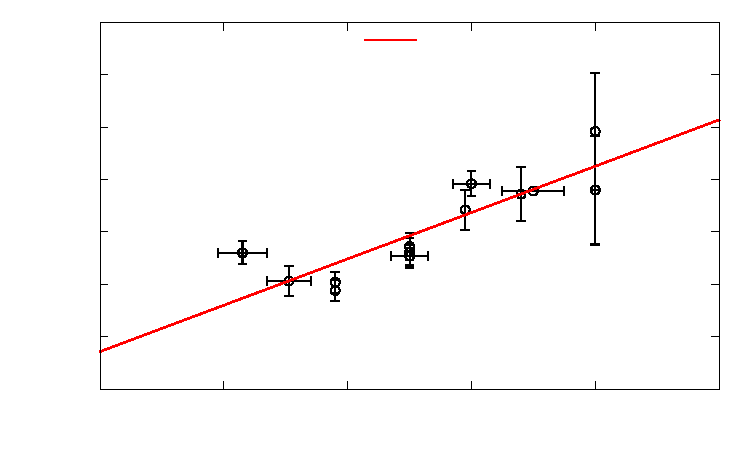
\includegraphics{GRAPH_Parameter_Fit_m-star_linear}}%
    \gplfronttext
  \end{picture}%
\endgroup

							}\endgroup
				\end{minipage}
				\begin{minipage}[c]{0.5\linewidth}
					\centering
						\begingroup\endlinechar=-1
							\resizebox{\textwidth}{!}{%
								% GNUPLOT: LaTeX picture with Postscript
\begingroup
  \makeatletter
  \providecommand\color[2][]{%
    \GenericError{(gnuplot) \space\space\space\@spaces}{%
      Package color not loaded in conjunction with
      terminal option `colourtext'%
    }{See the gnuplot documentation for explanation.%
    }{Either use 'blacktext' in gnuplot or load the package
      color.sty in LaTeX.}%
    \renewcommand\color[2][]{}%
  }%
  \providecommand\includegraphics[2][]{%
    \GenericError{(gnuplot) \space\space\space\@spaces}{%
      Package graphicx or graphics not loaded%
    }{See the gnuplot documentation for explanation.%
    }{The gnuplot epslatex terminal needs graphicx.sty or graphics.sty.}%
    \renewcommand\includegraphics[2][]{}%
  }%
  \providecommand\rotatebox[2]{#2}%
  \@ifundefined{ifGPcolor}{%
    \newif\ifGPcolor
    \GPcolortrue
  }{}%
  \@ifundefined{ifGPblacktext}{%
    \newif\ifGPblacktext
    \GPblacktexttrue
  }{}%
  % define a \g@addto@macro without @ in the name:
  \let\gplgaddtomacro\g@addto@macro
  % define empty templates for all commands taking text:
  \gdef\gplbacktext{}%
  \gdef\gplfronttext{}%
  \makeatother
  \ifGPblacktext
    % no textcolor at all
    \def\colorrgb#1{}%
    \def\colorgray#1{}%
  \else
    % gray or color?
    \ifGPcolor
      \def\colorrgb#1{\color[rgb]{#1}}%
      \def\colorgray#1{\color[gray]{#1}}%
      \expandafter\def\csname LTw\endcsname{\color{white}}%
      \expandafter\def\csname LTb\endcsname{\color{black}}%
      \expandafter\def\csname LTa\endcsname{\color{black}}%
      \expandafter\def\csname LT0\endcsname{\color[rgb]{1,0,0}}%
      \expandafter\def\csname LT1\endcsname{\color[rgb]{0,1,0}}%
      \expandafter\def\csname LT2\endcsname{\color[rgb]{0,0,1}}%
      \expandafter\def\csname LT3\endcsname{\color[rgb]{1,0,1}}%
      \expandafter\def\csname LT4\endcsname{\color[rgb]{0,1,1}}%
      \expandafter\def\csname LT5\endcsname{\color[rgb]{1,1,0}}%
      \expandafter\def\csname LT6\endcsname{\color[rgb]{0,0,0}}%
      \expandafter\def\csname LT7\endcsname{\color[rgb]{1,0.3,0}}%
      \expandafter\def\csname LT8\endcsname{\color[rgb]{0.5,0.5,0.5}}%
    \else
      % gray
      \def\colorrgb#1{\color{black}}%
      \def\colorgray#1{\color[gray]{#1}}%
      \expandafter\def\csname LTw\endcsname{\color{white}}%
      \expandafter\def\csname LTb\endcsname{\color{black}}%
      \expandafter\def\csname LTa\endcsname{\color{black}}%
      \expandafter\def\csname LT0\endcsname{\color{black}}%
      \expandafter\def\csname LT1\endcsname{\color{black}}%
      \expandafter\def\csname LT2\endcsname{\color{black}}%
      \expandafter\def\csname LT3\endcsname{\color{black}}%
      \expandafter\def\csname LT4\endcsname{\color{black}}%
      \expandafter\def\csname LT5\endcsname{\color{black}}%
      \expandafter\def\csname LT6\endcsname{\color{black}}%
      \expandafter\def\csname LT7\endcsname{\color{black}}%
      \expandafter\def\csname LT8\endcsname{\color{black}}%
    \fi
  \fi
  \setlength{\unitlength}{0.0500bp}%
  \begin{picture}(7200.00,4320.00)%
    \gplgaddtomacro\gplbacktext{%
      \put(849,595){\makebox(0,0)[r]{\strut{}-22}}%
      \put(849,947){\makebox(0,0)[r]{\strut{}-21.5}}%
      \put(849,1299){\makebox(0,0)[r]{\strut{}-21}}%
      \put(849,1651){\makebox(0,0)[r]{\strut{}-20.5}}%
      \put(849,2003){\makebox(0,0)[r]{\strut{}-20}}%
      \put(849,2355){\makebox(0,0)[r]{\strut{}-19.5}}%
      \put(849,2707){\makebox(0,0)[r]{\strut{}-19}}%
      \put(849,3059){\makebox(0,0)[r]{\strut{}-18.5}}%
      \put(849,3411){\makebox(0,0)[r]{\strut{}-18}}%
      \put(849,3763){\makebox(0,0)[r]{\strut{}-17.5}}%
      \put(849,4115){\makebox(0,0)[r]{\strut{}-17}}%
      \put(951,409){\makebox(0,0){\strut{} 0}}%
      \put(1611,409){\makebox(0,0){\strut{} 2}}%
      \put(2271,409){\makebox(0,0){\strut{} 4}}%
      \put(2932,409){\makebox(0,0){\strut{} 6}}%
      \put(3592,409){\makebox(0,0){\strut{} 8}}%
      \put(4252,409){\makebox(0,0){\strut{} 10}}%
      \put(4912,409){\makebox(0,0){\strut{} 12}}%
      \put(5573,409){\makebox(0,0){\strut{} 14}}%
      \put(6233,409){\makebox(0,0){\strut{} 16}}%
      \put(6893,409){\makebox(0,0){\strut{} 18}}%
      \csname LTb\endcsname%
      \put(144,2355){\rotatebox{-270}{\makebox(0,0){\strut{}Characteristic Magnitude ($M^*$)}}}%
      \csname LTb\endcsname%
      \put(3922,130){\makebox(0,0){\strut{}Redshift ($z$)}}%
      \put(3922,4022){\makebox(0,0){\strut{}}}%
    }%
    \gplgaddtomacro\gplfronttext{%
      \csname LTb\endcsname%
      \put(5877,1206){\makebox(0,0)[r]{\strut{}Predicated Value of $M^*$}}%
      \csname LTb\endcsname%
      \put(5877,1020){\makebox(0,0)[r]{\strut{}Upper Limit}}%
      \csname LTb\endcsname%
      \put(5877,834){\makebox(0,0)[r]{\strut{}Lower Limit}}%
    }%
    \gplbacktext
    \put(0,0){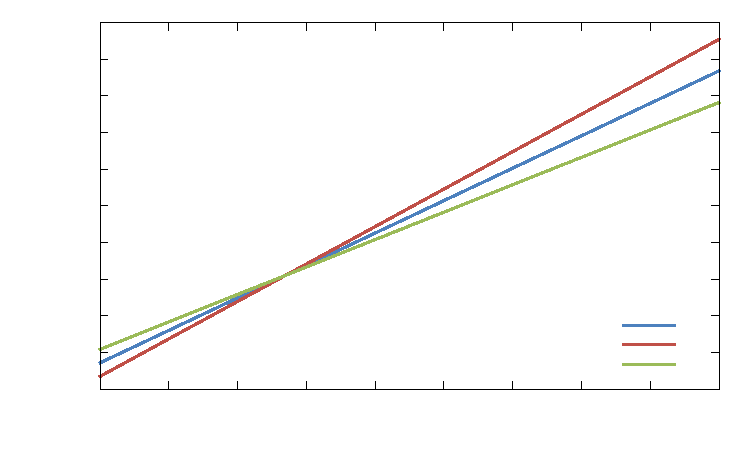
\includegraphics{GRAPH_Parameter_Fit_m-star_bounds}}%
    \gplfronttext
  \end{picture}%
\endgroup

							}\endgroup
				\end{minipage}
				\caption{The evolution of $M^{*}$ as a function of redshift according to past observational studies. Using the upper and lower limits of the parameter fit, the bounds of the value of $M^*$ are plotted, right.\label{fig:m-star_evolution}}
			\end{figure}
		% subsubsection linear_parameter_evolution_with_redshift (end)
% subsection parameter_evolution (end)

